\documentclass[12pt]{article}

\usepackage{amsmath}
\usepackage[super]{nth}
\usepackage[utf8]{inputenc}
\usepackage[T1]{fontenc}
\usepackage{textcomp}
\usepackage{gensymb}
\usepackage{graphicx}

\pagenumbering{arabic}

\begin{document}

\title{Graphical Analysis in ArtToMusic}
\date{December 06, 2016}
\author{Rafael De Smet}

\maketitle
\tableofcontents
\newpage
\section{Introduction}

In this paper I will be discussing several graphical analysis algorithms. Some of these are actually used in the code of ArtToMusic and others are discussed out of interest. I will also compare the algorithms I used and didn't use. These algorithms will return data which is used to generate music.

\section{Algorithms}

\subsection{Edge Detection}

Edge detection algorithms all use what are called convolution kernels. A kernel in image processing is a small matrix used to apply effects to an image, such as blurring, outlining. Here we will see kernels used for edge detection only. Listed below are six of the best and most used algorithms.

\begin{itemize}
        \item Sobel 
        \item Frei-Chen
        \item Prewitt
        \item Roberts Cross
        \item LoG
        \item Scharr
\end{itemize}

\subsubsection{Convolution kernel}

Since all the algorithms are based on the mathematical principle of convolution, an explanation of these convolution kernels is in order. 
\newline

Convolution is the technique of multiplying together two arrays of different size but of the same dimensionality. An array of dimensionality two is simply a matrix. When working with images the pixels are represented as a (2D) matrix and the kernel is also a 2D matrix.
The kernel is a small matrix that we will multiply with the image matrix to perform the convolution. This kernel matrix is different for each edge detection algorithm and we will see examples of different matrices in later chapters of this paper. 
\newline

Each pixel of the image is added to its local neighbours, weighted by the kernel. This produces a new image. If the kernel is chosen wisely, we get all the edges found in the image.
\newline

Mathematically we can write the convolution as follows, with $O$ the output image, $I$ the input image and $K$ the kernel:

\begin{equation}
O(i, j) =  \sum\limits_{k=1}^m\sum\limits_{l=1}^n I(i + k - 1, j + l - 1)K(k,l)
\end{equation}
\newline

An example will clarify the previous.

\begin{figure}[h]
\centering
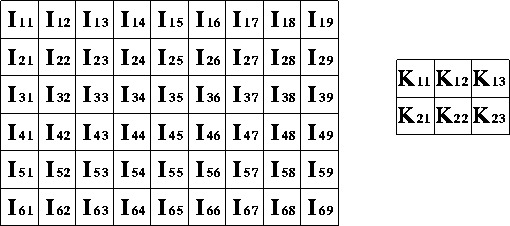
\includegraphics[scale = 0.5]{img/convolution}
\caption{A pixel matrix and a kernel}
\end{figure}

We expect an output image that shows us the edges of the original image. Using the kernel matrix we will compute every new pixel of the output image, by sliding the kernel matrix over the original pixels. Each kernel position corresponds to a sinle output pixel, the value of which is calculated by equation (1).

In our example, the value of the bottom right pixel in the output image will be found as follows:

\begin{equation}
O_{57} = I_{57}K_{11} + I_{58}K_{12} + I_{59}K_{13} + I_{67}K_{21} + I_{68}K_{22} + I_{69}K_{23}
\end{equation}
\newpage

In figure 2 you can see an idyllic landscape. We will use this image to see how well the different edge detection algorithms work.

\begin{figure}[h]
\centering
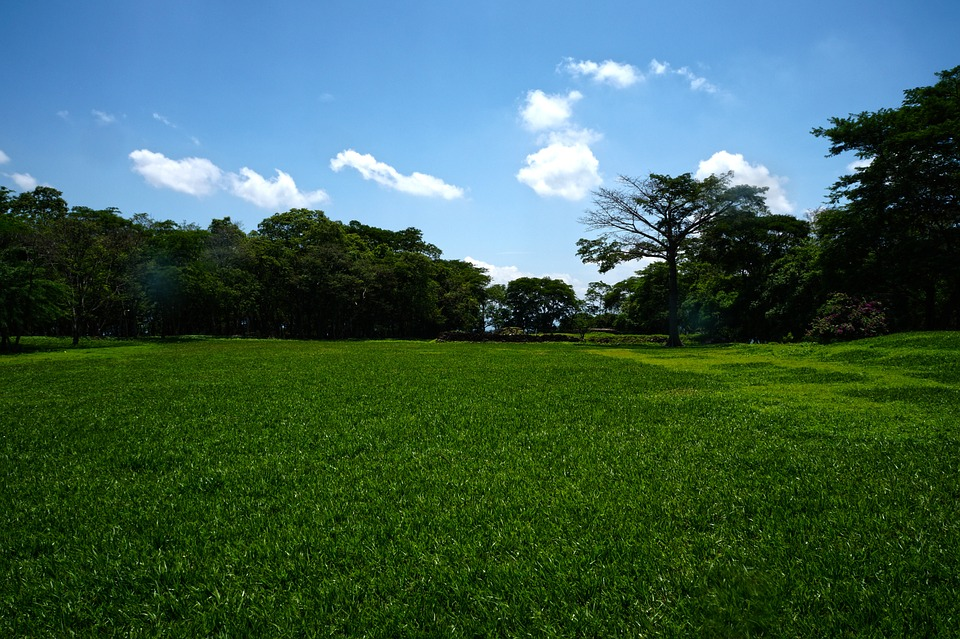
\includegraphics[scale = 0.3]{img/landscape}
\caption{Idyllic landscape}
\end{figure}

\subsubsection{Sobel}

 The Sobel algorithm performs a 2D spatial gradient measurement and finds regions of 'high spatial frequency' or edges. It uses two 3x3 kernels, one for the vertical edges and the other for the horizontal edges. These two kernels can be applied separately and afterwards combined to find all the edges.
 \newline

 The horizontal kernel: 
 $\begin{vmatrix}
        -1 & 0 & +1\\
        -2 & 0 & +2\\
        -1 & 0 & +1\\
\end{vmatrix}$
and the vertical kernel:
$\begin{vmatrix}
        +1 & +2 & +1\\
        0 & 0 & 0\\
        -1 & -2 & -1\\
\end{vmatrix}$

\begin{figure}[h]
\centering
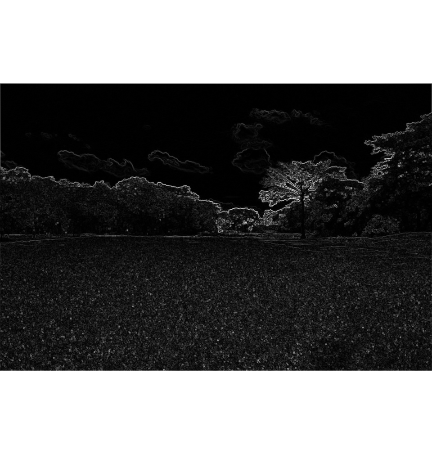
\includegraphics[scale = 0.45]{img/landscape_Sobel}
\caption{Sobel filter applied to Figure 2}
\end{figure}
\newpage

\subsubsection{Frei-Chen}
 The Frei-Chen algorithm also uses 3x3 kernels, but this time there are nine different convolution kernels. The four first matrices, G1, G2, G3, G4, are used for edges, the next four are used for lines and the last one is used to compute averages. 
\newline
\newline
 $G_1$ = $\frac{1}{2\sqrt2}$ $\begin{vmatrix}
        1 & \sqrt2 & 1\\
        0 & 0 & 0\\
        -1 & -\sqrt2 & -1\\
\end{vmatrix}$\hspace{5mm}
$G_2$ = $\frac{1}{2\sqrt2}$$\begin{vmatrix}
        1 & 0 & -1\\
        \sqrt2 & 0 & -\sqrt2\\
        1 & 0 & -1\\
\end{vmatrix}$\hspace{5mm}
$G_3$ = $\frac{1}{2\sqrt2}$$\begin{vmatrix}
        0 & -1 & \sqrt2\\
        1 & 0 & -1\\
        -\sqrt2 & 1 & 0\\
\end{vmatrix}$\hspace{5mm}
\newline
$G_4$ = $\frac{1}{2\sqrt2}$$\begin{vmatrix}
        \sqrt2 & -1 & 0\\
        -1 & 0 & 1\\
        0 & 1 & -\sqrt2\\
\end{vmatrix}$\hspace{5mm}
$G_5$ = $\frac{1}{2}$$\begin{vmatrix}
        0 & 1 & 0\\
        -1 & 0 & -1\\
        0 & 1 & 0\\
\end{vmatrix}$\hspace{10mm}
$G_6$ = $\frac{1}{2}$$\begin{vmatrix}
        -1 & 0 & 1\\
        0 & 0 & 0\\
        1 & 0 & -1\\
\end{vmatrix}$\hspace{5mm}
\newline
$G_7$ = $\frac{1}{6}$$\begin{vmatrix}
        1 & -2 & 1\\
        -2 & 4 & -2\\
        1 & -2 & 1\\
\end{vmatrix}$\hspace{13mm}
$G_8$ = $\frac{1}{6}$$\begin{vmatrix}
        -2 & 1 & -2\\
        1 & 4 & 1\\
        -2 & 1 & -2\\
\end{vmatrix}$\hspace{11mm}
$G_9$ = $\frac{1}{3}$$\begin{vmatrix}
        1 & 1 & 1\\
        1 & 1 & 1\\
        1 & 1 & 1\\
\end{vmatrix}$\hspace{5mm}

\begin{figure}[h]
\centering
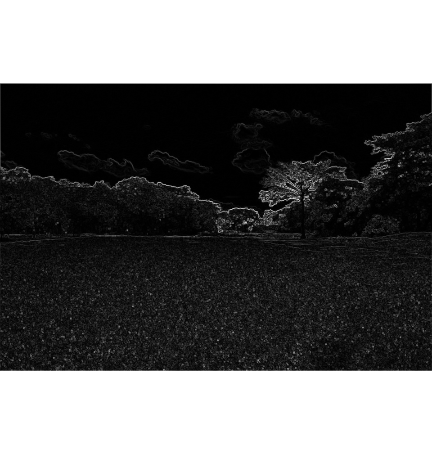
\includegraphics[scale = 0.45]{img/landscape_FreiChen}
\caption{Frei Chen filter applied to Figure 2}
\end{figure}
\newpage

\subsubsection{Prewitt}
This algorithm is very similar to the Sobel and Frei-Chen algorithms. Again, two kernels are used, one for the horizontal and one for the vertical edges. Afterwards, they are recombined to get all the edges in the image.
\newline

This time the kernels are considerably simpler:
\newline

Horizontal filter = $\begin{vmatrix}
        1 & 1 & 1\\
        0 & 0 & 0\\
        -1 & -1 & -1\\
\end{vmatrix}$\hspace{11mm}
Vertical filter = $\begin{vmatrix}
        -1 & 0 & 1\\
        -1 & 0 & 1\\
        -1 & 0 & 1\\
\end{vmatrix}$
\newline

\begin{figure}[h]
\centering
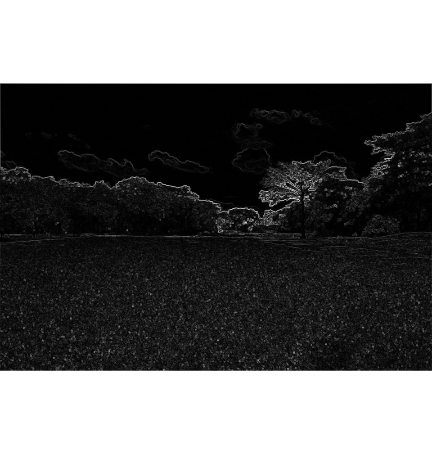
\includegraphics[scale = 0.45]{img/landscape_Prewitt}
\caption{Prewitt filter applied to Figure 2}
\end{figure}
\newpage

\subsubsection{Roberts Cross}
This algorithm uses even simpler kernels than Prewitt does. This time we use two 2x2 kernels. These kernels correspond to the edges running at 45° to the pixel grid, one for each of the two perpendicular orientations.
\newline

Horizontal filter = $\begin{vmatrix}
        1 & 0 \\
        0 & -1 \\
\end{vmatrix}$\hspace{11mm}
Vertical filter = $\begin{vmatrix}
        0 & 1\\
        -1 & 0\\
\end{vmatrix}$

\begin{figure}[h]
\centering
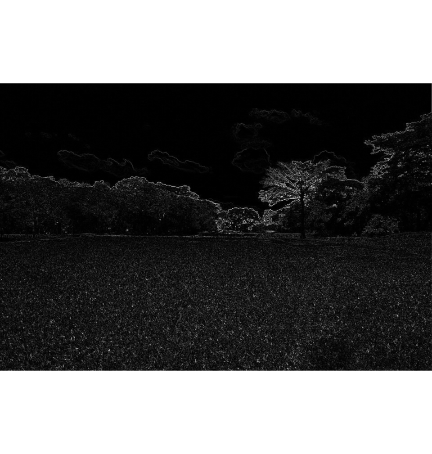
\includegraphics[scale = 0.45]{img/landscape_RobertsCross}
\caption{Roberts Cross filter applied to Figure 2}
\end{figure}

\subsubsection{LoG}
This algorithm combines two methods, the Gaussian filtering method\footnote{The Gaussian filter is used to blur images and remove noise and detail.} and the Laplacian method for edge detection\footnote{This method highlights regions in the image of rapid intensity change, so it is useful for edge detection.}. Hence the name "Laplacian of Gaussian" (LoG).
The edge points of an image are detected by finding the zero crossings of the \nth{2} derivative of the image intensity. Because the \nth{2} derivative is very sensitive to noise, which could give us bad results, the Gaussian filter is used to clear the noise from the image. 
\newline

The R library OpenImageR\footnote{https://cran.r-project.org/web/packages/OpenImageR/OpenImageR.pdf} uses the following LoG mask.
\newline

LoG mask = $\begin{vmatrix}
        1 & 1 & 1\\
        1 & -8 & 1\\
        1 & 1 & 1\\
\end{vmatrix}$

\begin{figure}[h]
\centering
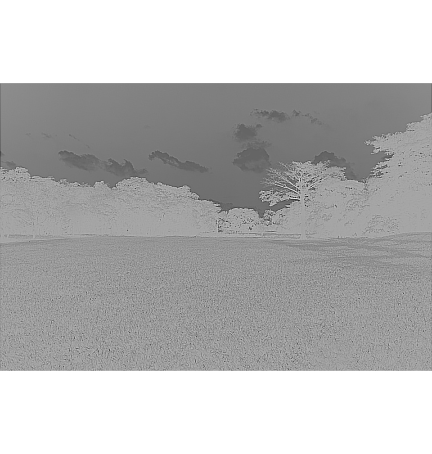
\includegraphics[scale = 0.45]{img/landscape_LoG}
\caption{LoG filter applied to Figure 2}
\end{figure}

\subsubsection{Scharr}
This algorithm is an extension of the Sobel algorithm. Although the Sobel kernels are very good, they do not have perfect rotational symmetry. This is what the Scharr kernels try to optimize.
\newline

The most frequently used kernels are the following:
\newline

Horizontal filter = $\begin{vmatrix}
        3 & 10 & 3\\
        0 & 0 & 0\\
        -3 & -10 & -3\\
\end{vmatrix}$\hspace{11mm}
Vertical filter = $\begin{vmatrix}
        3 & 0 & -3\\
        10 & 0 & -10\\
        3 & 0 & -3\\
\end{vmatrix}$\hspace{5mm}

\begin{figure}[h]
\centering
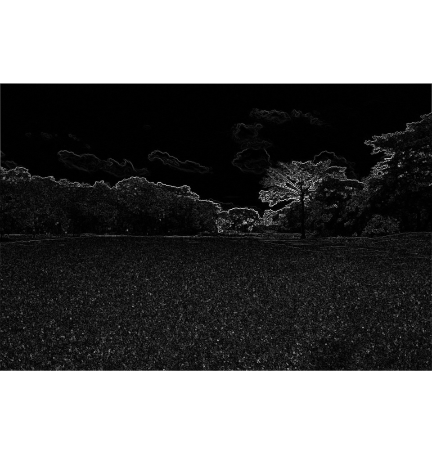
\includegraphics[scale = 0.45]{img/landscape_Scharr}
\caption{Scharr filter applied to Figure 2}
\end{figure}
\newpage

\subsection{Color Analysis}
Only edge detection algorithms are not sufficient to get enough data from the image to form a musical interpretation. We will need some form of color analysis. This section describes some algorithms and methods we can use to obtain information about the colors of the image.

\subsubsection{RGB - HSV - CMYK}
This is the most common representation of color on a computer. Each pixel is described using three values, the amount of red (R), green (G) and blue (B). Using these values we can count how many pixels in the image are dominantly red, green or blue. When we're going to translate the image data into musical patterns, we can match each color to another kind of music (happy, sad, etc...)
\newline

HSV, sometimes called HSB, is another representation of a pixel. This time we use the hue (H), the saturation (S) and the brightness or value (B or V) to describe the pixel. Where the RGB model consists of three values indicating the amounts of a certain color each pixel has, the HSV model consists of three independent components. 
\newline

First we have the hue, which is basically the color. Here the color is represented using a circle with all the colors on it. The value of this component is the degrees of the angle we have to make on the circle to get this color.  

The saturation indicates the fullness of the color. This value is expressed in a percentage, with 0\% a gray, flat color and 100\%  a full, rich color.

The value or brightness indicates the lightness of the color and is also expressed in a percentage, 0\% is black and 100\% is white.

This representation will be used in combination with the RGB model in the translation into the musical patterns.
\newline

\begin{figure}[h]
\centering
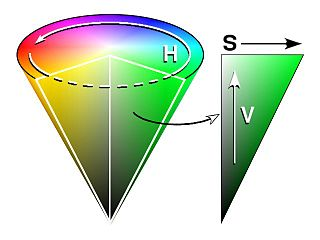
\includegraphics[scale = 0.45]{img/hsv}
\caption{The HSV color representation}
\end{figure}

CMYK is another representation of color, based on the mixing of four colors, cyan (C), magenta (M), yellow (Y) and key (K, black). This model is used frequently with printing.
\newline

When combined, the data from the three models can be very accurate to use in the translation to music.

\subsubsection{Black And White Balance}
During the image analysis we will convert the image to a gray scale image, so we can determine the amount of white and black in it. Using the RGB model, this is an easy process. Black in the RGB model is (0,0,0) and white is (255,255,255). So we can simply count the amount of pixels that are very close to those two values and we know the amount of black and white pixels in the image.
\newline

Analogous to this we can count every gray pixel in the image, by finding every pixel where the RGB values are exactly the same.

\subsubsection{Color Quantization - Image Segmentation}

Sometimes it can be easier to work with images that are partitioned in simpler regions. This technique is called image segmentation or color quantification. There are many different ways to implement this technique. One such simple approach is using the k-means cluster algorithm. This algorithm attempts to partition a data set into k clusters. The data set contains the RGB values of each pixel.

In R this can be done easily. The code to do this is in the file segmentation.R\footnote{Code found on https://www.r-bloggers.com/color-quantization-in-r/}.
\newline

A second technique is the X-means algorithm which is an improvement of the k-means algorithm. Where we don't know how many clusters there are when using k-means, and thus guessing, the X-means algorithm can determine the number of clusters by itself.

\subsection{Image Hashing}
It is also possible to get the hash value of an image. This is a hexadecimal number.

\subsubsection{Average Hashing}
The first hash method is just the average hash (aHash) of the image. This algorithm works in four steps.

\begin{enumerate}
        \item Convert the image to grayscale. 
        \item Reduce the size of the image, to reduce the number of computations.
        \item Average the resulting colors. For an 8x8 image, 64 will be averaged.
        \item Compute the bits of the hash value by comparing if each color value is above or below the mean.
        \item Construct the hash.
\end{enumerate}

\subsubsection{Difference Hash}
We can also compute the dHash of an image. It is similar to the average hash, but now the difference between adjacent pixels is also considered in the computation.

\subsubsection{Perceptive Hash}
This method uses the discrete cosine transform (DCT) and compares the pixels based on the frequencies, given by the DCT, instead of the color values.

DCT is very similar to Fourier analysis, it expresses a finite sequence of points, in this case the pixels, in terms of a sum of cosine functions.

\subsubsection{Use Of The Hash}
One application of these methods is the recognition of images. Search engines like Google use this technique to search similar images as any image you provide to the search engine. I could use this as a way to store information about the image my application has already scanned and generated music for.
\newline

For example, if you use a picture of a tree with the ArtToMusic application, it will produce a certain kind of music. If you use another picture of another tree that looks quite similar to the first tree, you expect to get a similar result in the music. The hash values of the images will help with this. 

\subsection{Entropy}

\subsubsection{Image}

Another method we can use to get information from an image is via entropy.
The entropy of an image is a measure of the amount of disorder in the image. This technique is also used in other disciplines, for example to study the structures of living organisms.
\newline

When talking about images, we consider the following. If all the pixels of the image have the same level, the entropy is zero. This means there is not a lot of information (almost none) to be gained from the image. When all the pixels in the image are different, the entropy of this image is maximum and there is a lot of information to get from the image.
As the entropy describes how much (dis)order there is, we will use this to determine how much (dis)order there is in the generated music.
\newline

To get the right information about the pixels, we use a histogram that shows the count of the distinct pixel values. 
\newline

The entropy of an image $H$ is defined as:
\begin{equation}
H = - \sum_{k=0}^{M-1} p_k log_2 (p_k)
\end{equation}

where M is the number of distinct pixel values and $p_k$ is the count of each pixel level.
\newline

You can calculate the entropy of an image, but it is more useful to calculate the entropy of an analysis of that picture. This gives us information about the analysis and not just the image in general.

\begin{thebibliography}{1}

\bibitem{OpenImageR} Lampros Mouselimis {\em OpenPackageR, An Image Processing Toolkit} 2017

\bibitem{Convolution} R. Fisher, S. Perkins, A. Walker, E. Wolfart {\em Hypermedia Image Processing Reference} 2003

\bibitem{Frei_Chen_Sobel} Daniel R\'akos' blog (http://rastergrid.com/blog/2011/01/frei-chen-edge-detector/) 2011

\bibitem{Gaussian} University of Auckland, New Zealand, Computer Science course Computer Graphics and Image Processing {\em Gaussian Filtering} 2010

\bibitem{edge} Computaç\~ao Visual e Multimédia, course on Image Processing

\bibitem{prewitt} RoboRealm blog {http://www.roborealm.com/help/Prewitt.php} 2017

\bibitem{image filter} Simon Colton, Pedro Torres {\em Evolving Approximate Image Filters} 2009, Computational Creativity Group
Department of Computing, Imperial College London

\bibitem{hash} Dr. Neal Krawetz' blog (http://www.hackerfactor.com/blog/?/archives/529-Kind-of-Like-That.html) 2013

\bibitem{entropy} John Loomis' site (http://www.johnloomis.org/ece563/notes/basics/entropy/entropy.html) 1998

\bibitem{entropy} Kevin Meurer's blog (http://kevinmeurer.com/a-simple-guide-to-entropy-based-discretization/) 2015

\bibitem{color} Ryan Walker's blogpost (https://www.r-bloggers.com/color-quantization-in-r/) 2016

\end{thebibliography}

\end{document}
